%\section{Protocol} \fxnote{Did we want to add something about asking them about the pain after each methods? or what did we discuss about this}
%This protocol will describe the present study, which consist of two experiments testing pain tolerance and pain threshold after practicing mindfulness meditation or after not practicing mindfulness meditation. 

%\section{Purpose}
%The treatment of chronic pain has constraints, as the treatments are only relieving the pain instead of curing the pain. Another issue is that some of these treatments, example medication, have side effect, as described in \secref{sec:treatment}. 
%There is alternative to medication such as yoga, hypnosis and physical therapy, psychological therapy and chiropractor, which have shown to have an influence on relieving pain. But these treatments are often used in combination with pharmaceutical treatment. Furthermore, most of these alternative require an external person to apply, which can result in high costs, as mention in \secref{sec:treatment}.
%An alternative to the present treatment is mindfulness meditation, which have shown an effect on relieving conditions as stress, depression and  anxiety through the ability to enhance emotion regulation, cognitive control, acceptance and positive mood, as described in \secref{sec:SOTA}. 
%Different studies have shown that practicing meditation have an effect on reliving pain. However, these studies have most often investigated long-term mindfulness meditation for patient with eater chronic pain or low back pain. There is a limit on studies that have investigated short-term in patient with neck pain, why this could be interesting to investigate further, as approximately 25\% of the chronic pain patients suffer from this condition. In order to investigated the influence of mindfulness meditation on pain threshold and pain tolerance for people with neck pain following hypothesis is proposed:

%Approximately 375 million people suffer from chronic neck pain. The primary treatment for those patients is medication. But medication has side effects, as described in \secref{sec:treatment}.  Besides medication, alternative treatment methods are used, often in combination with medication. For example physical therapy, chiropractor or psychological therapy showed a positive influence on pain relief. Most of the alternative treatment methods are related with high costs, because they require a specialist for the application. Whereas mindfulness meditation can be practiced alone. Hence a lot of studies focused on the ability of mindfulness meditation to relieve pain.
%As mentioned in \secref{sec:SOTA}, there are not many studies which show the effect of mindfulness meditation on chronic neck pain. Since a lot of people suffer from chronic neck pain this study investigates the influence of mindfulness meditation on neck pain. %Pain levels of chronic pain patients are not very easy to access and to quantify, therefore pressure pain was applied with an algometer on healthy subjects, 

%Pain levels of chronic pain patients are not very easy to access and to quantify because the pain is neuropathic and the assessment is multidimensional and the experience of pain is subjective. Therefore, in order to get some quantifiable measures on pain to clarify if mindfulness meditation will have an effect on sensitivity of pain, acute pain in the form of pressure pain was applied to healthy subjects. If the pressure pain tolerance is increased, after practicing mindfulness meditation, in the upper trapezius it might also have an effect on pain in other body parts. And if it is possible to show an effect on acute pain due to an increase in the tolerance on healthy subjects it might also be possible to help relieving pain in chronic pain patients. On basis of this the study wants to test the following hypothesis:

%***** This part should be more convincing ****
%Pain levels of chronic pain patients are not very easy to access and to quantify because the assessment of neuropathic pain is multidimensional and the experience of chronic pain is subjective. Also variation of the patients' pain from day to day and throughout the day makes it difficult to get reliable and comparable  values of the pain levels of these patients. Therefore acute pressure pain was applied with an algometer to healthy subjects to get quantifiable values of pain and test the following hypothesis: 
%*** Until here ***


%\textit{Short-term mindfulness meditation practice increases the pressure pain threshold and the pressure pain tolerance in the upper trapezius.}

%\vspace{-.5cm}
%\begin{itemize}
%\item Short-term mindfulness meditation increases the pressure pain threshold and the pressure pain tolerance.
%\end{itemize}

\section{Subjects}
%Forty healthy subjects were recruited for the experiment, 20 males (M) and 20 females (F) with a mean age $\pm$XX. A homogeneous group of participants were enrolled in order to limit the amount of variables in the study. For insuring this, specific inclusion and exclusion criteria have been formed for this experiment. 
42 healthy subjects were recruited for the experiment, 21 males and 21 females, with a mean age of 23.93 $\pm$ 2.74 years. To get a homogeneous group of participants, specific inclusion and exclusion criteria were  formed for this experiment.

\textbf{Inclusion criteria:}
\vspace{-.5cm}
\begin{itemize}
	%\item Healthy
	\vspace{-.3cm}
	\item Age between 20 and 35 years
	\vspace{-.3cm}
	\item No obesity 
	\vspace{-.3cm}
	\item Time to meditate for 5 days, 20 minutes per day
\end{itemize}

\textbf{Exclusion criteria:}
\vspace{-.5cm}
\begin{itemize}
	\item Ongoing meditation practice 
	\vspace{-.3cm}
	\item Acute or chronic pain
	\vspace{-.3cm}
	\item Pregnancy 
	\vspace{-.3cm}
	\item Neurological, musculoskeletal or mental illness
	\vspace{-.3cm}
	\item Drug or alcohol abuse
	\vspace{-.3cm}
	\item Medication with antidepressant or analgesic properties
	\vspace{-.3cm}
	\item Lack of ability to cooperate
\end{itemize}

\vspace{-.5cm}
%Furthermore, is it not necessary that subjects believe in the effect of mindfulness meditation.\fxnote{I don't know about this sentence, i think it does not fit in here. Maybe it is more something we should write for the participants or could we put it in as one of our criteria?.}

\section{Study design} 
%For this particular experiment a parallel study was conducted. The subjects recruited for the experiment were randomly assigned in two different groups, the control group or the treatment group, with a equal amount of female and males in the groups. The control group consisted of twenty subjects no meditation. The treatment group consisted of twenty subjects meditation. The structure of the study design is illustrated on \figref{fig:studydesign}. 
%For this particular experiment a random controlled study was conducted. 

The subjects, recruited for the experiment, were assigned into different groups, treatment and control group. Whereby an equal gender distribution was strove. The treatment group was measured before and after the intervention, which was the practice of mindfulness FA meditation. To ensure that a detected effect was not due to habituation to the measurements, a control group was measured with the same time difference in between. Moreover, to minimize bias, the examiner was blinded. The structure of the study design is illustrated in \figref{fig:studydesign}.

\begin{figure}[H]
	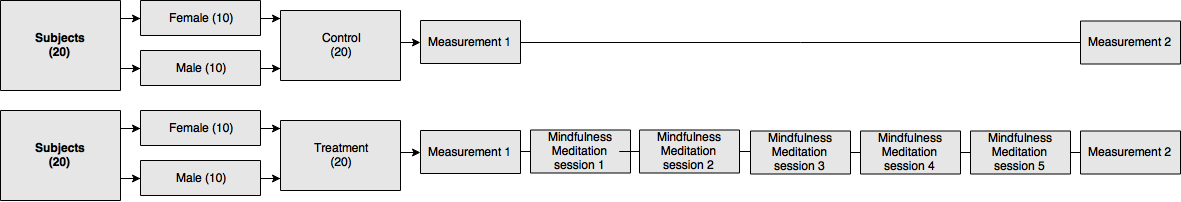
\includegraphics[width=1\textwidth]{figures/studydesign.png} 
	\caption{Parallel study design, whereby subjects were assigned into treatment and control group striving an equal gender distribution. The treatment group was meditating on 5 consecutive days between the measurements, whilst the control group continued their normal routine.}
	\label{fig:studydesign}  
\end{figure}  

%There will be seven to eight days between the measurements. The treatments groups start practicing mindfulness meditation three or four days after the first measurement and will then practice mindfulness meditation for five days and will on the last day of meditation be measured again.

%\section{Setup}
%The Pressure Pain Threshold (PPT), defined as the pressure at which the sensation changed from pressure to pain, has been recognized as an effective and reliable way to quantify pain measures. In this study PPT was measured using Wagner Force Ten$^{TM}$ Digital force Gage. PPT were measured in the upper trapezius. Testing points were marked to ensure reliable and rapid location during the experimental procedure. 
%The algometer was applied four times, two on the left side and two on the right side of the upper trapezius, and the average of the registrations was filed. The subjects had a 5 minutes resting time between measurements. PPT values were measured two times, the first day of the study and after 5 days since the first measure.

%\subsubsection{Mindfulness meditation}
%The treatment group should do guided meditation for 30 minutes in small groups for 5 days. On the first day the mediators would be giving a short introduction to mindfulness meditation. During the meditation the subjects would be in a sitting position with the face  away from the other subjects, to assure that they would not get distracted. 


\section{Procedure}
Firstly general information about the subjects were collected, which are illustrated in \tabref{tab:subjectsA} and \tabref{tab:subjectsB} in Appendix \ref{SubjectINFO}. Furthermore, information about the experimental procedure was given to the subjects. The measurement point was marked at the right upper trapezius, as illustrated in \figref{fig:trapezius}, while the subject laid prone, to ensure reliable and rapid location during the experimental procedure. 
The location on the right upper trapezius was determined by the midpoint between the acromion and 7th cervical vertebra. The distance was notated, so the same location could be used for each measurement session. 

\begin{figure}[H]
	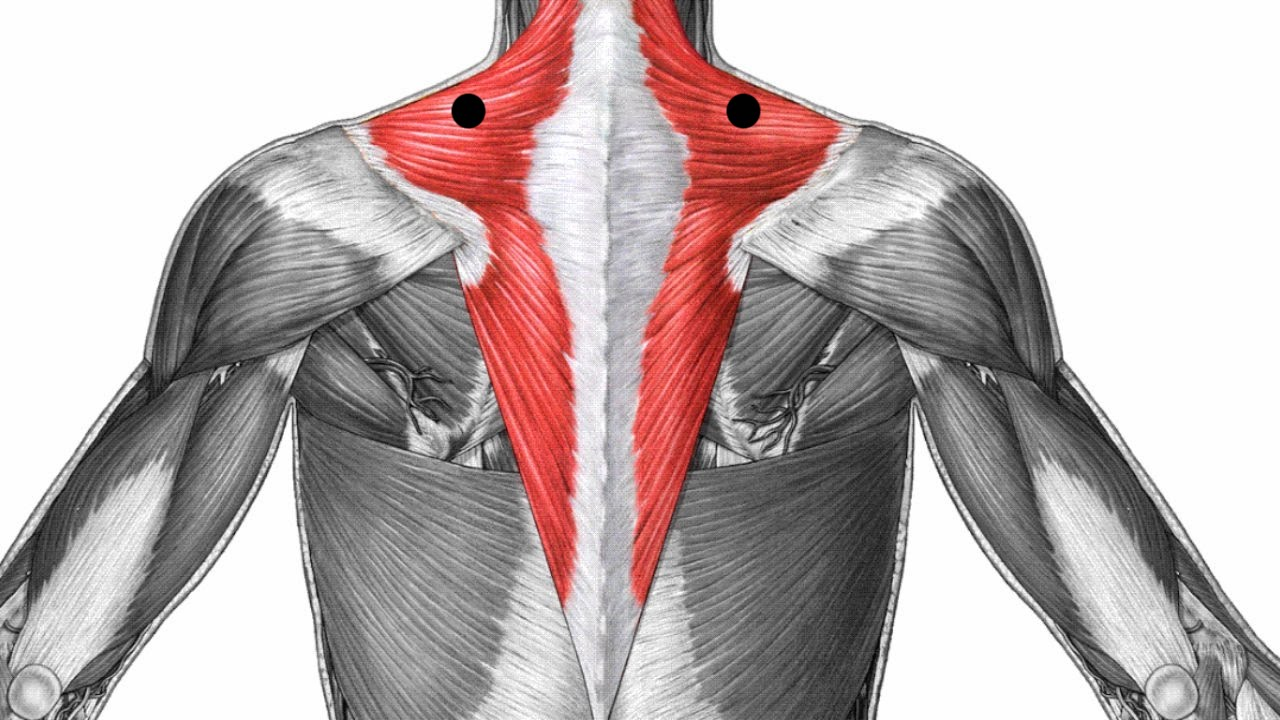
\includegraphics[width=0.5\textwidth]{figures/trapezius} 
	\caption{The measurement point on the right upper trapezius is marked with a black dot.}
	\label{fig:trapezius}  
\end{figure}  

Threshold and Tolerance were measured with an algometer (Wagner Force Ten ™  Digital force Gage). During the use of the algometer it was considered that the pressure application should be conducted steady and consistent \cite{Fischer1987, Kinser2009}, wherefore the examiner underwent a brief training with the algometer before the beginning of the experiment \cite{ Kinser2009, Vaughan2007}. 

Firstly, Threshold was measured, therefore the algometer was applied until the subject begins to feel the first sign of pain or discomfort. Secondly, Tolerance was measured at the same point and the pressure was applied until the maximum level of pain that the subject could stand was reached. Those measurements rely on the ability of the subjects to rate their own pain, hence the measurements were repeated three times to get representative values of Threshold and Tolerance. The average of these measurements was used for Threshold and Tolerance. To avoid hyperesthesia, there was 5 minutes pause in between the repetitions. 

To test the effect of mindfulness FA meditation on Threshold and Tolerance, the treatment group practiced 20 minutes mindfulness FA meditation on 5 consecutive days. To ensure the same meditation conditions for all of the subjects, a guided meditation in form of an audio file was used. The used audio file was created as a combination of a recording of a guided mindfulness FA meditation and Buddhist meditation music for positive energy. The Buddhist meditation music is playing in the background consistently. From time to time guidance through the mindfulness FA meditation is provided by a male voice, which explains in the beginning to focus the attention on the sensations of breathing and reminds the subjects from time to time to bring the focus back to the breath. The complete content of the used audio file can be seen in Appendix \ref{FAM}.

In the beginning of each meditation session subjects were told to have the most comfortable position during the meditation.  Additionally a short introduction to mindfulness FA meditation was provided orally on the first day. 

The subjects of the control group continued their normal routine.
After the last meditation session of the treatment group the second measurement session was conducted. The same time interval between the measurements were used for the subjects of the control group. The second measurement session was conducted likewise the first measurement session.


\section{Data Analysis}
First a Shapiro-Wilk test was applied to evaluate the normality of the samples. Thereby the sample scores are compared with the scores, which are anticipated under normal distribution. The Shapiro-Wilk test has shown to be valid even in small samples (n < 20), wherefore it was chosen for this study. \cite{Shapiro1965,Mooi2018} Afterwards a Levene’s test was applied to evaluate the equality of variances.

According to the outcome of the Shapiro-Wilk test and the Levene’s test, the parametric tests ANOVA and t-test were chosen.
The two-way mixed ANOVA was used in this study, whereby factor 1 denotes the group of subjects, either treatment or control group, and factor 2 denotes the measurement session, either the first (Pre) or the second (Post). Therewith it was evaluated, if there is a statistical significant difference between those data samples, i.e. 
two kinds of variations were evaluated, the between-subjects variation in factor 1 and the within-subjects variation in factor 2. 
Threshold and Tolerance have been analyzed with separate two-way mixed ANOVAs. \cite{Mooi2018}

The t-test was used to compare the changes in Threshold and Tolerance between the measurement sessions of both, treatment and control group. Therefore the difference relative to Pre measurement (relative difference) in Threshold and Tolerance between the Pre and Post measurement was calculated for each subject. A t-test was applied to test the mean difference between treatment and control group’s relative difference \cite{Mooi2018}. The relative difference of Threshold and Tolerance have been tested separately. 

%According to the outcome of the Shapiro-Wilk test either a non-parametric or a parametric test was chosen.
%For comparison of treatment and control group with regards to threshold and tolerance of first and second measurement a Kruskal-Wallis test was applied in the case of a non-normal distribution and a two-way mixed ANOVA was applied in the case of a normal distribution.

% *** Add something about the factors we are using ***
 
%For comparison of treatment and control group with regards to the difference in threshold and tolerance as a percentage of first and second measurement a Mann-Whitney-U test was applied in the case of a non-parametric distribution and a t-test was applied in the case of a normal distribution. 

%*** Why you would also like to analyze the data in another way, and how the percentage exactly is defined.  Explain it more ***


